\documentclass[fleqn,10pt]{wlpeerj}
\title{Overview and comparison of open source solutions for storing spatial-temporal numerical arrays}

\author[1]{Martin Jung}
\affil[1]{Current address:  School of Life Sciences, University of Sussex, Brighton BN1 9QG, UK.  }

\keywords{Spatial-temporal, GIS, database, raster analysis}

\begin{abstract}
Dummy abstract text. Dummy abstract text. Dummy abstract text. Dummy abstract text. Dummy abstract text. Dummy abstract text. Dummy abstract text. Dummy abstract text. Dummy abstract text. Dummy abstract text. Dummy abstract text.
\end{abstract}

\begin{document}

\flushbottom
\maketitle
\thispagestyle{empty}

\section*{Introduction}

Intention. Relevance of remote-sensing data to ecology, conservation, food security

example with multispectral landsat data.

same machine, different ways

zodb, postgres, rasdaman
scidb,rasterlite
rds files, hdf and netcdf files
folder
postgres pointcloud extension
https://github.com/pgpointcloud/pointcloud


Difficulties is that spatial-temporal data has 4 dimensions

make figure of different ways for storage (time-voxel, simple table)

Although propertiary solutions for storing spatial-temporal raster dataset exists such as ... - we will focus explicitly on solutions that are freely available, reproducible and might find application in small to medium size research settings.

We will also focus on comparably small settings such for small-medium scientific or business settings, recognizing that larger solutions for clusters  might exist \citep{Winslett}

In this paper current methods and their individual shortcoming and merits of storing spatial-temporal raster images with open-source products is discussed. 
Furthermore we will test and evaluate the individual methods in the light of speed, storage efficiency and ease of management.

We identify four main purposes of establishing a database system - which are management, storage, query and subset
modularity (as expansion of data and functions) and 


\section*{Some \LaTeX{} Examples}
\label{sec:examples}

Use section and subsection commands to organize your document. \LaTeX{} handles all the formatting and numbering automatically. Use ref and label commands for cross-references.

because hardware speed is relative and subject to computational power we will make the comparison as being relative to a simple on-disk storage of files. 
Obviously some RIO speeds might also change depending on improvements in code

Idea: Store only change of pixels in a temporal fashion. Baseline complete, then only change
Likely only practiable for classifed rasters
Define temporal resolution in advance, then write association if change happened
maybe store the change in a formula

comparison between database types


\subsection*{Figures and Tables}


Use the table and tabular commands for basic tables --- see Table~\ref{tab:widgets}, for example. You can upload a figure (JPEG, PNG or PDF) using the project menu. To include it in your document, use the includegraphics command as in the code for Figure~\ref{fig:view} below.

spatiallite only stores numbers, but not date types


\begin{figure}[ht]
\centering
%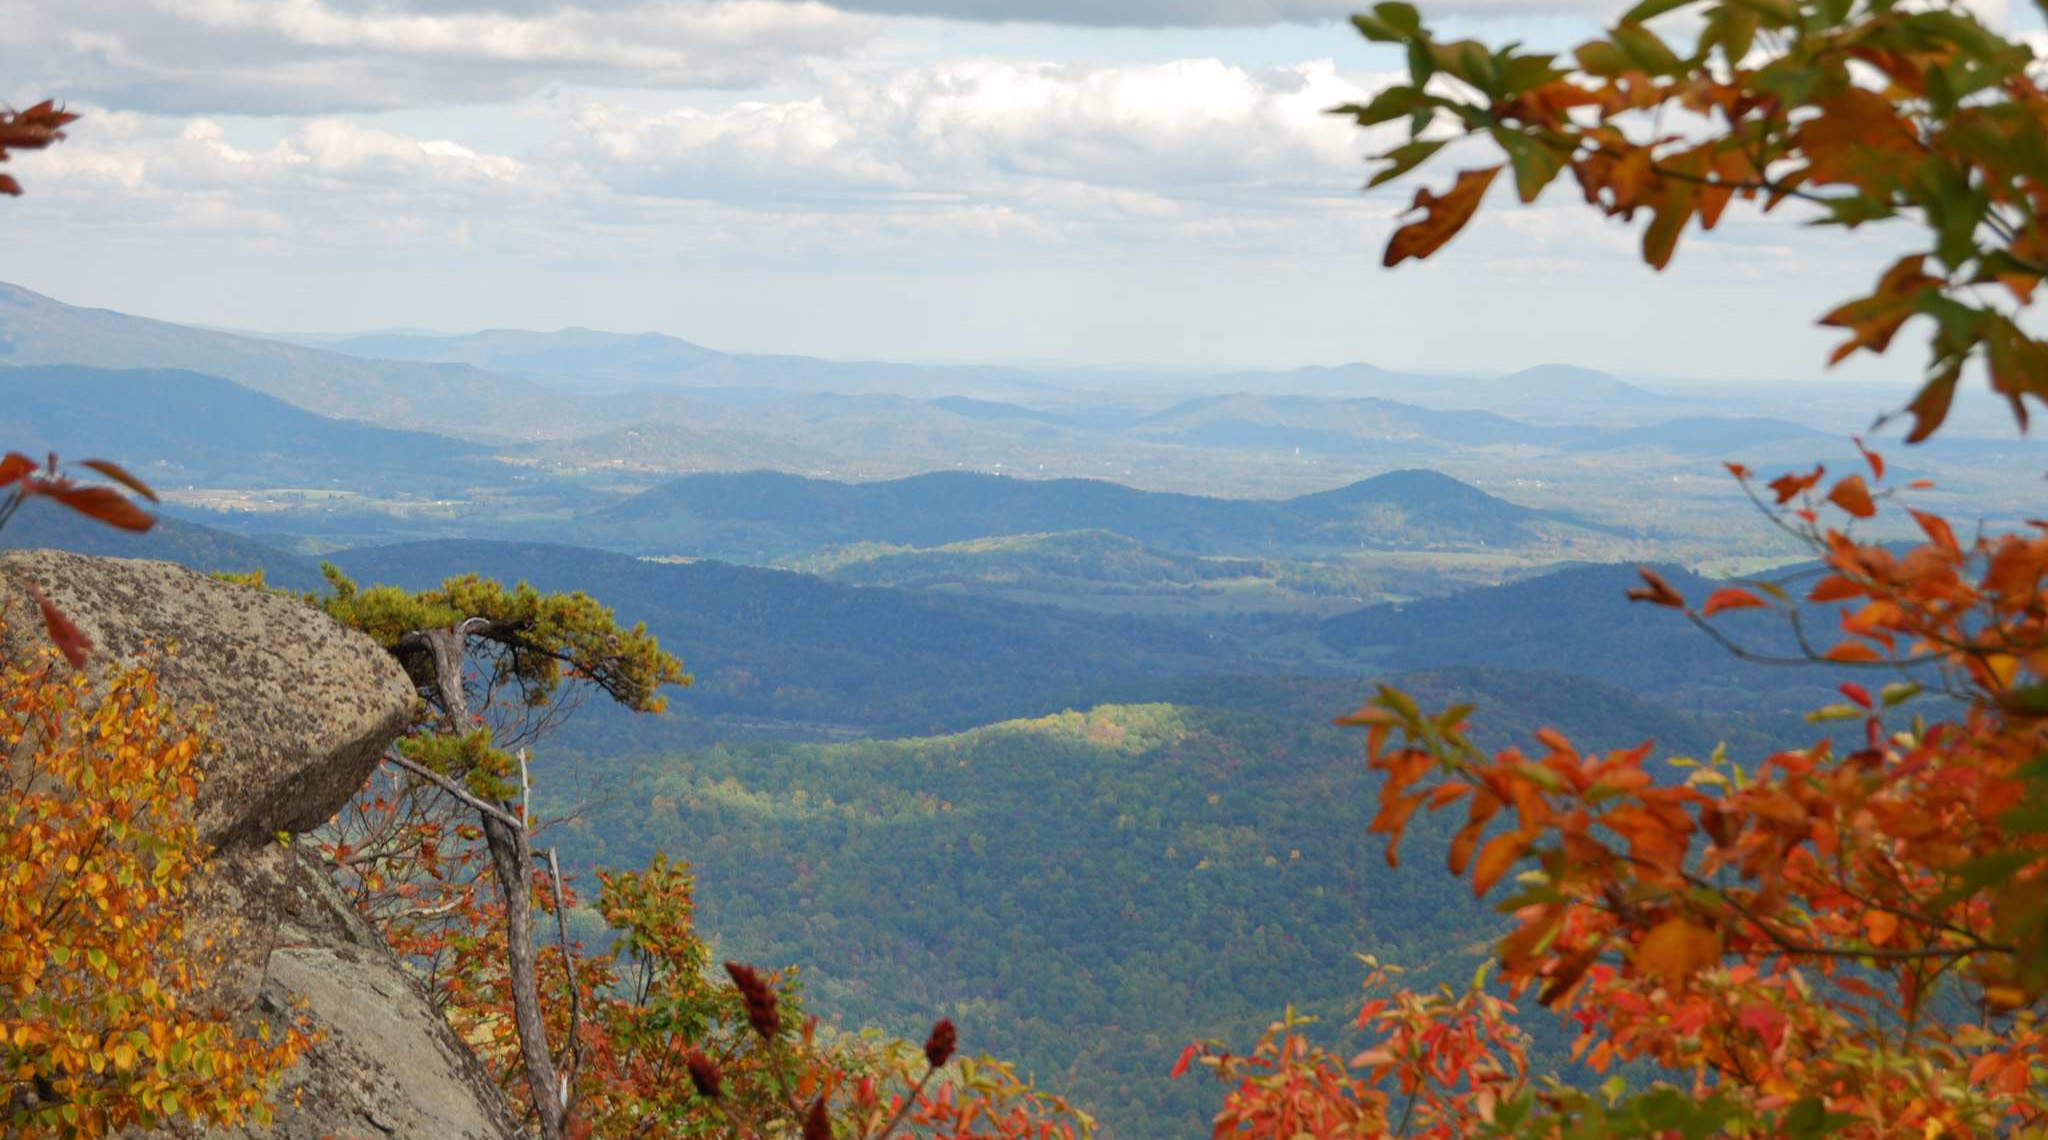
\includegraphics[width=\linewidth]{view}
\caption{An example image.}
\label{fig:view}
\end{figure}

\begin{table}[ht]
\centering
\begin{tabular}{l|r}
Item & Quantity \\\hline
Widgets & 42 \\
Gadgets & 13
\end{tabular}
\caption{\label{tab:widgets}An example table.}
\end{table}

\subsection*{Citations}

LaTeX formats citations and references automatically using the bibliography records in your .bib file, which you can edit via the project menu. Use the cite command for an inline citation, like \cite{Figueredo:2009dg}, and the citep command for a citation in parentheses \citep{Figueredo:2009dg}.

\subsection*{Mathematics}

\LaTeX{} is great at typesetting mathematics. Let $X_1, X_2, \ldots, X_n$ be a sequence of independent and identically distributed random variables with $\text{E}[X_i] = \mu$ and $\text{Var}[X_i] = \sigma^2 < \infty$, and let
$$S_n = \frac{X_1 + X_2 + \cdots + X_n}{n}
      = \frac{1}{n}\sum_{i}^{n} X_i$$
denote their mean. Then as $n$ approaches infinity, the random variables $\sqrt{n}(S_n - \mu)$ converge in distribution to a normal $\mathcal{N}(0, \sigma^2)$.

\subsection*{Lists}

You can make lists with automatic numbering \dots

\begin{enumerate}[noitemsep]
\item Like this,
\item and like this.
\end{enumerate}
\dots or bullet points \dots
\begin{itemize}[noitemsep]
\item Like this,
\item and like this.
\end{itemize}
\dots or with words and descriptions \dots
\begin{description}
\item[Word] Definition
\item[Concept] Explanation
\item[Idea] Text
\end{description}

We hope you find write\LaTeX\ useful for your PeerJ submission, and please let us know if you have any feedback. Further examples with dummy text are included in the following pages.

\section*{Methods}

\lipsum[4] % Dummy text

\begin{equation}
\cos^3 \theta =\frac{1}{4}\cos\theta+\frac{3}{4}\cos 3\theta
\label{eq:refname2}
\end{equation}

\lipsum[5] % Dummy text

\subsection*{Subsection}

\lipsum[6] % Dummy text

\paragraph{Paragraph} \lipsum[7] % Dummy text
\paragraph{Paragraph} \lipsum[8] % Dummy text

\subsection*{Subsection}

\lipsum[9] % Dummy text

\begin{figure}[ht]\centering
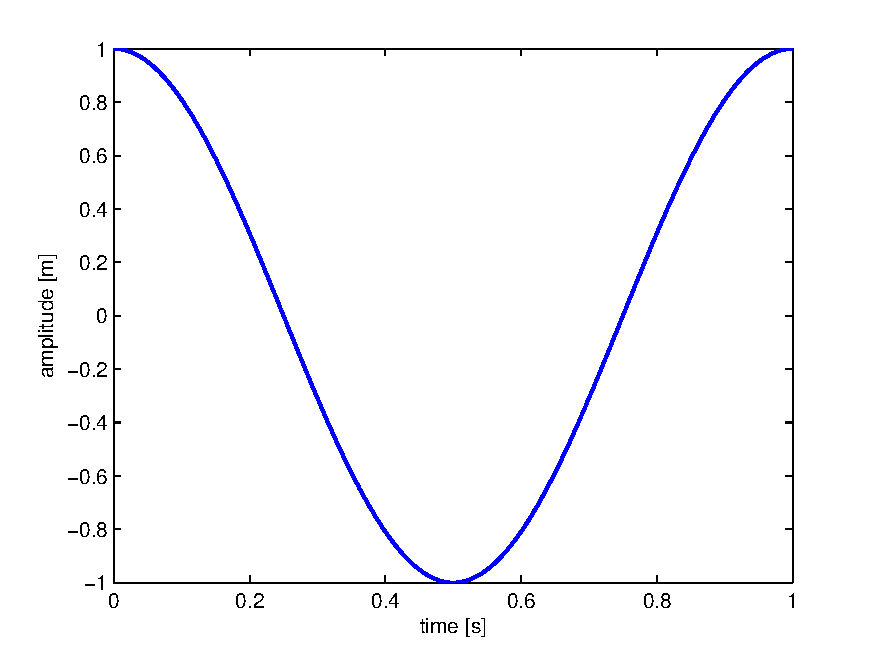
\includegraphics[width=\linewidth]{results}
\caption{In-text Picture}
\label{fig:results}
\end{figure}

Reference to Figure \ref{fig:results}.

\section*{Results and Discussion}

\lipsum[10] % Dummy text

\subsection*{Subsection}

\lipsum[11] % Dummy text

\subsubsection*{Subsubsection}

\lipsum[12] % Dummy text

\subsubsection*{Subsubsection}

\lipsum[14] % Dummy text

\subsection*{Subsection}

\lipsum[15-20] % Dummy text

\section*{Acknowledgments}



\bibliography{bib}

\end{document}
